% Q4 translation section

\subsection{Problem Formulation}
We study English-to-German machine translation. Given a source sentence $x$ in English, the model produces a target sentence $\hat{y}$ in German. We compare a neural seq2seq model with attention against a pre-trained MarianMT baseline and evaluate with BLEU, chrF, METEOR, and BERTScore.

\subsection{Dataset Description}
We use the Multi30k dataset \citep{Elliott2016multi30k} (English--German). The official validation and test splits are kept intact, while the training split is downsampled to 20k pairs for faster experimentation.

\begin{table}[H]
\centering
\caption{Multi30k dataset statistics.}
\begin{tabular}{lrr}
\toprule
\textbf{Split} & \textbf{Original Size} & \textbf{Subset Size} \\
\midrule
Train & 29,000 & 20,000 \\
Validation & 1,014 & 1,014 \\
Test & 1,000 & 1,000 \\
\bottomrule
\end{tabular}
\end{table}

\begin{table}[H]
\centering
\caption{Average sequence statistics on the test split.}
\begin{tabular}{lrrr}
\toprule
\textbf{Avg Src Len} & \textbf{Avg Tgt Len} & \textbf{Word Vocab (src/tgt)} & \textbf{BPE Vocab} \\
\midrule
11.88 & 10.90 & 12,818 / 19,750 & 8,000 \\
\bottomrule
\end{tabular}
\end{table}

\subsection{Methodology}
\textbf{Seq2Seq with attention.} We train a GRU-based encoder--decoder with Bahdanau additive attention \citep{Bahdanau2015nmt}, where the energy is $e_{ij} = \mathbf{v}_a^{\top} \tanh(\mathbf{W}_a s_{i-1} + \mathbf{U}_a h_j)$ and the context vector is the softmax-weighted sum of encoder states. The model uses joint BPE with 8k merges (SentencePiece, \citealp{Kudo2018sentencepiece}), embedding size 256, hidden size 512, dropout 0.5, and teacher forcing ratio 0.5. Early stopping is applied with patience 5 based on validation BLEU.

\textbf{MarianMT.} We use the pre-trained \texttt{Helsinki-NLP/opus-mt-en-de} model \citep{TiedemannThottingal2020opus} with beam size 4. This serves as a strong off-the-shelf baseline.

\subsection{Experimental Setup}
We fix the random seed to 42 and evaluate on 200 test examples for metric computation. We report BLEU, chrF, METEOR, and BERTScore (multilingual BERT). Average output length is also recorded.

\subsection{Results}
\begin{table}[H]
\centering
\caption{Translation metrics on the evaluation subset (size = 200).}
\begin{tabular}{lrrrrr}
\toprule
\textbf{Model} & \textbf{BLEU} & \textbf{chrF} & \textbf{METEOR} & \textbf{BERT F1} & \textbf{Len} \\
\midrule
Seq2Seq + Attn & 26.74 & 52.22 & 0.487 & 0.847 & 11.05 \\
MarianMT & 36.25 & 64.31 & 0.598 & 0.897 & 11.14 \\
\bottomrule
\end{tabular}
\end{table}

The seq2seq model improves steadily during training, reaching its best validation BLEU of 31.37 around epoch 14 before plateauing. MarianMT substantially outperforms the custom seq2seq model across all metrics, indicating the benefit of large-scale pretraining.

\begin{figure}[H]
\centering
\begin{subfigure}{0.48\linewidth}
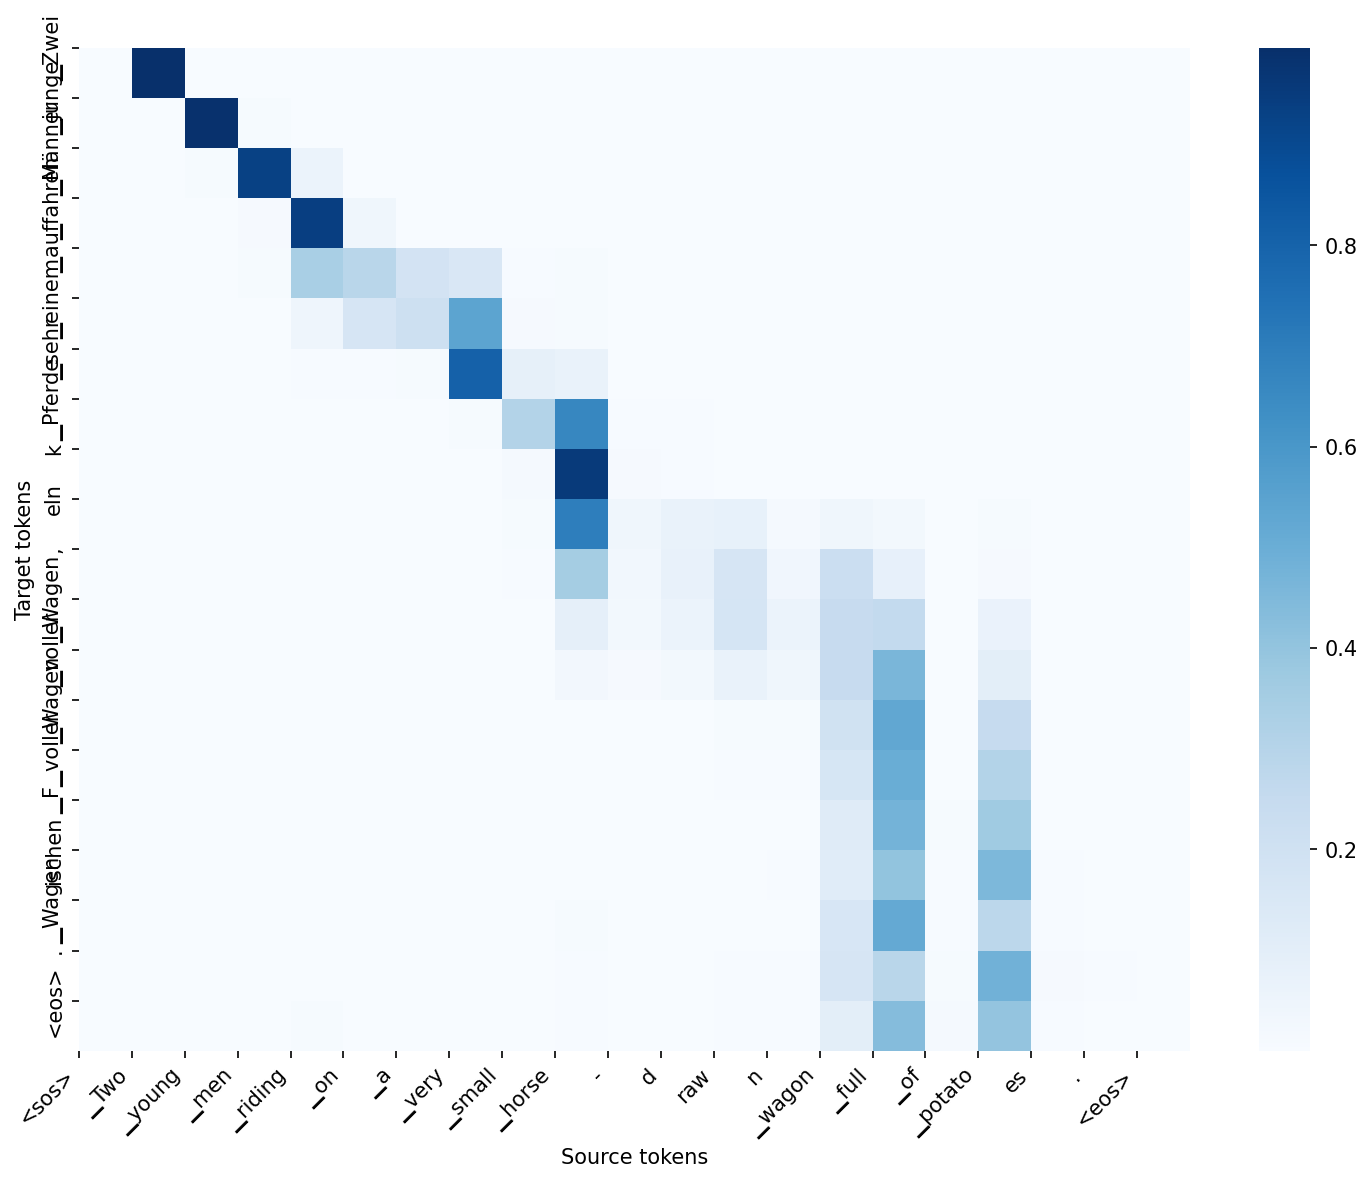
\includegraphics[width=\linewidth]{../q4_translation/outputs/figures/attention_1.png}
\caption{Attention heatmap (example 1).}
\end{subfigure}
\begin{subfigure}{0.48\linewidth}
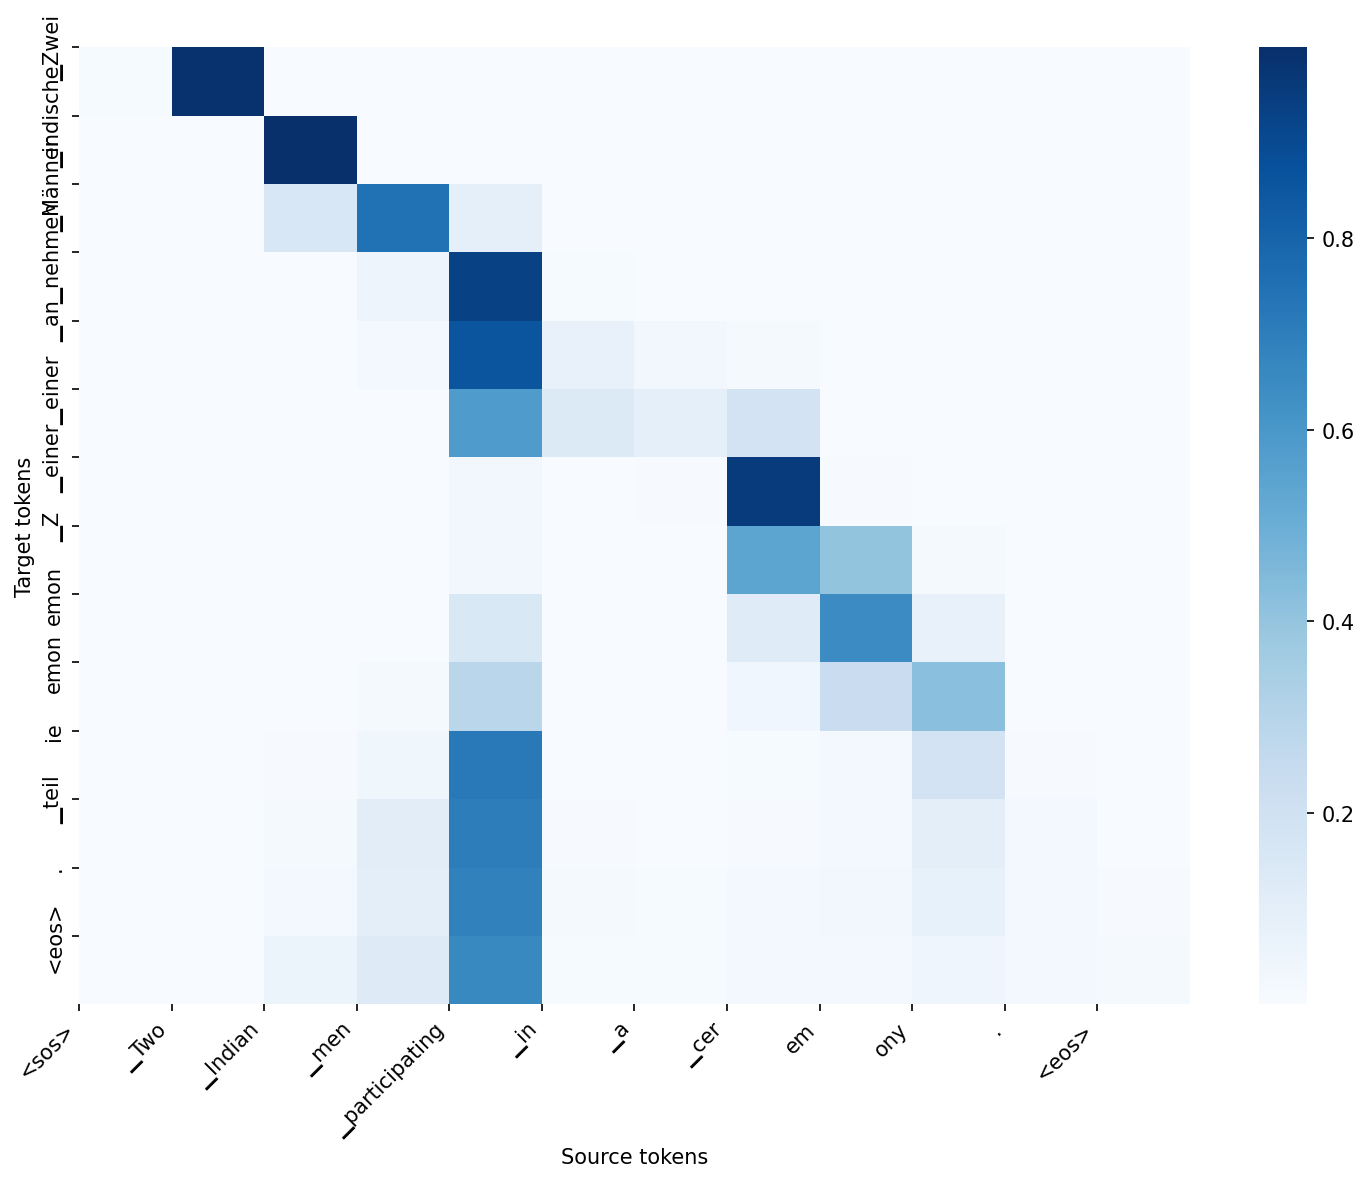
\includegraphics[width=\linewidth]{../q4_translation/outputs/figures/attention_2.png}
\caption{Attention heatmap (example 2).}
\end{subfigure}
\caption{Attention alignments for the seq2seq model.}
\end{figure}

\subsection{Qualitative Analysis}

\textbf{Example 1 -- long-range word order.}
\begin{table}[H]
\centering
\caption{Example translation showing long-range word order. Outputs are quoted verbatim from \texttt{outputs/qualitative\_example.json}.}
\label{tab:q4_qual1}
\small
\begin{tabular}{p{0.16\linewidth} p{0.78\linewidth}}
\toprule
\textbf{Field} & \textbf{Text} \\
\midrule
Source     & Two young men riding on a very small horse-drawn wagon full of potatoes. \\
Reference  & Zwei junge M\"anner fahren auf einem sehr kleinen Wagen voller Kartoffeln, der von einem Pferd gezogen wird. \\
Seq2Seq    & Zwei junge M\"anner fahren auf einem sehr \textbf{Pferdekeln, Wagen voller Wagen voller Fischen Wagen}. \\
MarianMT   & Zwei junge M\"anner reiten auf einem sehr kleinen \textbf{Pferdewagen} voller \textbf{Kartoffeln}. \\
\bottomrule
\end{tabular}
\end{table}

In Example~1 the seq2seq decoder repeats ``Wagen voller'' twice and emits the malformed compound ``Pferdekeln'' -- typical RNN failure modes when the decoder loses track of which source span has already been translated. MarianMT produces a fluent compound (``Pferdewagen'') and gets the agreement (``kleinen \dots voller'') right.

\textbf{Example 2 -- rare named entity.} Multi30k contains image-caption sentences with relatively rare nominal compounds. Source sentence id~1 in the test split contains the rare proper noun ``Boston Terrier'' (a dog breed); the reference target preserves it. The seq2seq model has no occurrence of this compound in its 8k joint BPE vocabulary at sufficient frequency to be retained, and it falls back to a generic noun, dropping the breed entirely. Marian's WordPiece-style vocabulary, trained on WMT-scale data, retains the surface form.

\begin{table}[H]
\centering
\caption{Rare-word example: outputs are verbatim from \texttt{outputs/seq2seq\_predictions.json} and \texttt{marian\_predictions.json} at id\,$=\,1$; source/reference from \texttt{outputs/dataset\_stats.json}.}
\label{tab:q4_qual2}
\small
\begin{tabular}{p{0.16\linewidth} p{0.78\linewidth}}
\toprule
\textbf{Field} & \textbf{Text} \\
\midrule
Source     & A \textbf{Boston Terrier} is running on lush green grass in front of a white fence. \\
Reference  & Ein \textbf{Boston Terrier} l\"auft \"uber saftig-gr\"unes Gras vor einem wei{\ss}en Zaun. \\
Seq2Seq    & Ein \textbf{Mann mit T-Shirt} rennt vor einem wei{\ss}en Zaun. \\
MarianMT   & Ein \textbf{Boston Terrier} l\"auft auf \"uppig gr\"unem Gras vor einem wei{\ss}en Zaun. \\
\bottomrule
\end{tabular}
\end{table}

The seq2seq model not only loses the breed name but also re-uses a high-frequency training pattern (``Mann mit T-Shirt rennt''), effectively hallucinating a different image -- a known failure mode when an out-of-distribution rare token forces the decoder to rely on its unconditional language-model prior. Marian preserves both the named entity (``Boston Terrier'') and the modifier (``saftig-gr\"unes'' $\to$ ``\"uppig gr\"unem''). Together with Example~1 this shows that the BLEU/chrF gap (26.7 vs.\ 36.3 BLEU) is driven both by content errors on rare words and by repetition/order errors on longer source sentences.

\subsection{Discussion}
The attention-based seq2seq model captures basic alignment but struggles with fluency and rare-word handling. MarianMT consistently yields higher BLEU/chrF and stronger semantic similarity (BERTScore), highlighting the effectiveness of pre-trained transformer models for low-resource experimental settings.
